\documentclass[10pt,a4paper,twocolumn]{article}
\usepackage[T1]{fontenc}
\usepackage[utf8]{inputenc}
\usepackage[brazil]{babel}
\usepackage{lmodern}
\usepackage[margin=1.55cm,columnsep=0.65cm]{geometry}
\usepackage{amsmath,amssymb,booktabs,graphicx,microtype,url}
\usepackage[font=small,labelfont=bf]{caption}
\usepackage[hidelinks]{hyperref}
\usepackage{enumitem,needspace}
\setlist{nosep,leftmargin=*}
\setlength{\parindent}{1em}
\setlength{\parskip}{.12em}
\setlength{\textfloatsep}{8pt plus 2pt minus 2pt}
\setlength{\intextsep}{7pt plus 2pt minus 2pt}
\title{Mini-projeto: buscas clássicas e otimização contínua}
\author{Resolução comentada e experimentos reproduzíveis}
\date{Enunciado de 25 de agosto de 2026}
\begin{document}
\maketitle
\vspace{-1.6em}
\begin{abstract}\noindent
Implementam-se busca em largura (BFS), busca gulosa Best-First e uma versão gulosa otimizada para transformar sequências binárias por inversões de intervalos de custo unitário. Demonstra-se que o custo ótimo é a quantidade de blocos de diferenças. Em seguida, implementa-se gradiente descendente projetado e propõe-se uma penalização diferenciável para mudanças não consecutivas. Experimentos reproduzíveis com 30 pares por tamanho cobrem $L=2,4,\ldots,4096$; a BFS é medida apenas até $L=16$ devido à explosão combinatória.
\end{abstract}
\vspace{-.8em}
\section{Buscas clássicas}
\textbf{Problema e operações.} Dadas duas sequências binárias $s,t\in\{0,1\}^L$, pode-se inverter um bit isolado ou qualquer intervalo inclusivo $[i,j]$, pagando uma unidade em ambos os casos. A subrotina implementa
\[
F_{i,j}(s)_k=\begin{cases}1-s_k,&i\le k\le j,\\s_k,&\text{caso contrário.}\end{cases}
\]
Definindo $d=s\oplus t$, as posições com $d_k=1$ são as diferenças a corrigir. O exemplo pedido é
\begin{center}\ttfamily\footnotesize
00001001000011001100111\\
00000000000000000000000
\end{center}
Os blocos de diferenças são $[5,5]$, $[8,8]$, $[13,14]$, $[17,18]$ e $[21,23]$ (índices iniciados em 1). Invertê-los nessa ordem produz, respectivamente,
\begin{center}\ttfamily\scriptsize
00000001000011001100111\\
00000000000011001100111\\
00000000000000001100111\\
00000000000000000000111\\
00000000000000000000000
\end{center}
Logo, o custo é $5$.

\textbf{BFS.} A fila FIFO começa em $s$. Para cada estado retirado, geram-se os $L(L+1)/2$ intervalos possíveis, armazenando um predecessor e o intervalo utilizado apenas quando o estado ainda não foi visitado. Ao retirar $t$ da fila, reconstrói-se a trajetória. Como todas as arestas têm custo unitário, a BFS retorna um caminho mínimo, com custo igual ao número de operações. O espaço de estados tem $2^L$ elementos; a complexidade máxima é $O(2^L L^2)$ em tempo e $O(2^L)$ em memória.

\textbf{Heurística e gulosa.} Adota-se
\[
\boxed{h(s)=\#\{\text{blocos máximos de 1 em }s\oplus t\}.}
\]
Justificativa: acrescente zeros virtuais nas extremidades de $d$ e marque suas transições $0\leftrightarrow 1$. Se há $r$ blocos de 1, há $2r$ transições. Uma inversão de intervalo altera somente as duas transições de suas extremidades, reduzindo $r$ no máximo em $1$. Portanto, são necessários ao menos $r$ passos. Inverter cada bloco de 1 usa exatamente $r$ passos, logo $h(s)=r$ é o custo restante \emph{exato}, e não apenas uma estimativa. A busca gulosa Best-First mantém uma fila de prioridade ordenada por $h$; há sempre um sucessor com $h-1$, portanto o caminho escolhido tem custo ótimo. A implementação otimizada pula a enumeração de vizinhos e inverte diretamente os blocos detectados em uma varredura, com complexidade $O(L)$ para obter os intervalos. As três versões retornam operações e custo; a BFS e a Best-First explícita só são executadas em tamanhos viáveis.

\section{Experimentos de busca}
Para cada comprimento $L\in\{2,4,8,\ldots,4096\}$, geraram-se $N=30$ pares binários independentes, com gerador NumPy e semente $2026$. Mediram-se custos, estados expandidos e tempos com \texttt{perf\_counter}; resultados completos e código acompanham este relatório. Todos os pares testados pelas três versões tiveram o mesmo custo ótimo. Na Tabela~\ref{tab:result}, ``--'' indica experimento \emph{não executado}, e não tempo zero.
\begin{table}[h]
\centering\caption{Médias de 30 pares por comprimento; tempo em milissegundos.}\label{tab:result}
\scriptsize\setlength{\tabcolsep}{3.5pt}
\begin{tabular}{rrrrr}
\toprule
$L$ & custo & BFS (ms) & Gulosa (ms) & Otim. (ms)\\
\midrule
2    & 0,90   & 0,0021 & 0,0072 & 0,0012\\
4    & 1,13   & 0,0062 & 0,0216 & 0,0013\\
8    & 2,47   & 0,3091 & 0,1683 & 0,0018\\
16   & 4,00   & 280,382 & 1,3750 & 0,0032\\
32   & 8,23   & -- & -- & 0,0048\\
64   & 15,73  & -- & -- & 0,0070\\
128  & 32,83  & -- & -- & 0,0136\\
256  & 63,27  & -- & -- & 0,0287\\
512  & 128,10 & -- & -- & 0,0522\\
1024 & 257,93 & -- & -- & 0,1130\\
2048 & 512,57 & -- & -- & 0,2111\\
4096 & 1027,77& -- & -- & 0,4070\\
\bottomrule
\end{tabular}
\end{table}
A BFS expandiu, em média, $2{,}87$, $7{,}07$, $153{,}23$ e $28.349{,}53$ estados para $L=2,4,8,16$; a Best-First expandiu $1{,}9$, $2{,}13$, $3{,}47$ e $5$ estados. Para pares independentes com bits equiprováveis, $d$ também é equiprovável e $\mathbb{E}[h]=(L+1)/4$, próximo das médias observadas. Tempos muito pequenos dependem da máquina e do overhead de medição; a comparação estrutural é mais robusta.
\begin{figure}[h]
\centering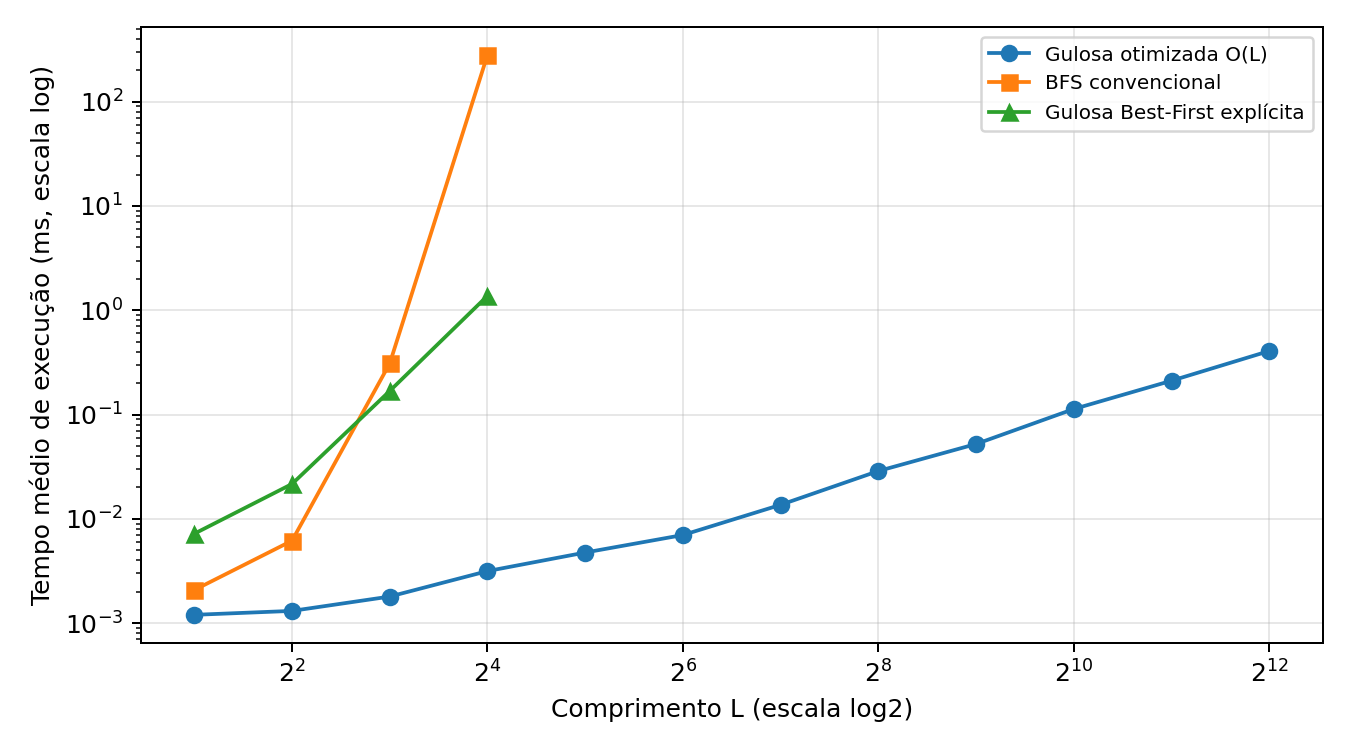
\includegraphics[width=\columnwidth]{resultados/grafico_tempo.png}
\caption{Tempo por tamanho. Não se extrapolam tempos de BFS para tamanhos não medidos.}
\end{figure}
\begin{figure}[h]
\centering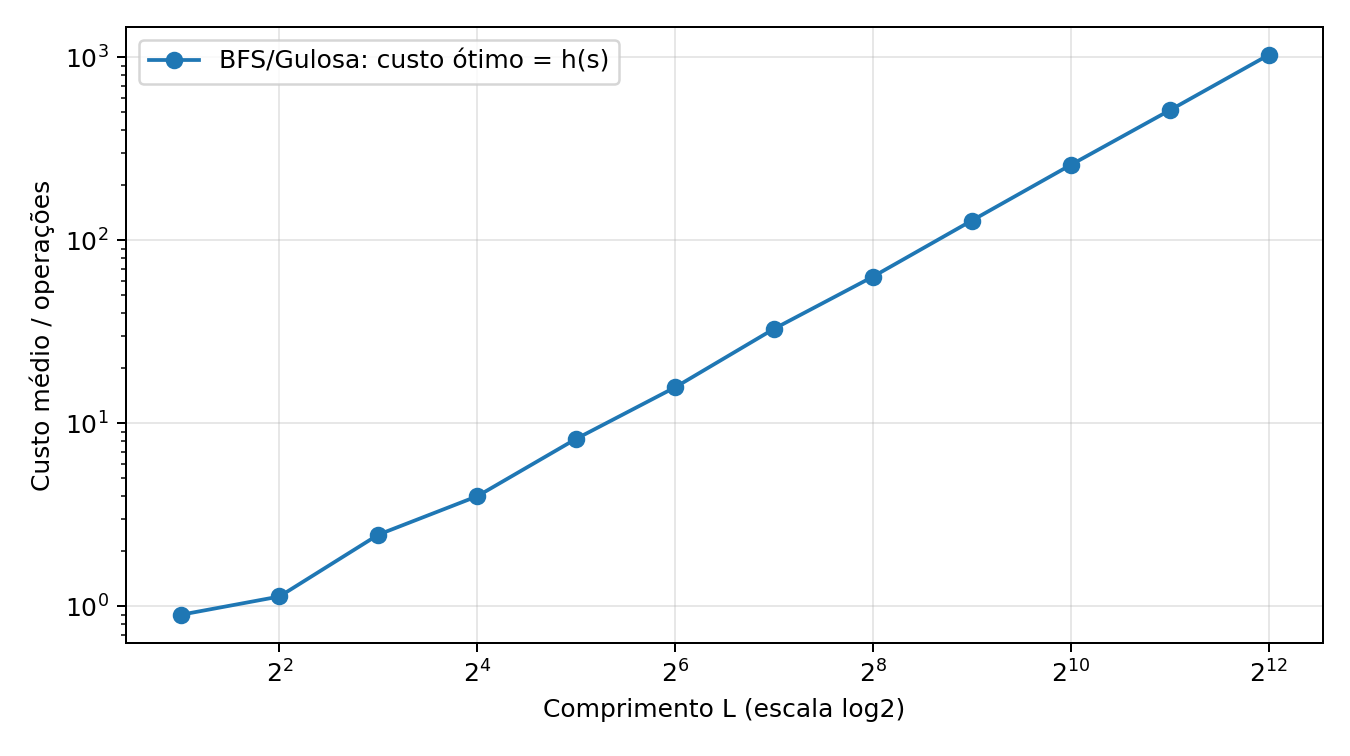
\includegraphics[width=\columnwidth]{resultados/grafico_custo.png}
\caption{Custo ótimo médio, comum às abordagens; nos comprimentos grandes foi calculado pela gulosa otimizada.}
\end{figure}

\section{Gradiente descendente}
\textbf{Relaxamento e erro.} Representamos cada bit por $x_i\in[0,1]$, sendo $x^{(0)}$ o vetor binário inicial e $y$ o vetor alvo. Minimiza-se a função do enunciado
\[
\mathcal{L}(x)=\sum_{i=1}^L(x_i-y_i)^2,\qquad
\nabla\mathcal{L}(x)=2(x-y).
\]
Alcançar $\mathcal{L}=0$ equivale a alcançar o alvo no espaço contínuo; converter de volta a bits é feito por limiar $x_i\ge 0{,}5$. A trajetória discreta de flips não é imposta pelo erro quadrático: a função apenas aproxima o vetor final, sem preferência por alterações consecutivas. No gradiente simples,
\[
x^{(k+1)}=x^{(k)}-2\eta(x^{(k)}-y),\quad
\Delta x^{(k)}=x^{(k+1)}-x^{(k)}.
\]
O código retorna a sequência completa desses vetores $\Delta x^{(k)}$. Para um bit inicial $1$, alvo $0$ e $\eta=0{,}45$, as três primeiras mudanças são $-0{,}9$, $-0{,}09$ e $-0{,}009$. Sem projeção, $x^{(1)}=1-2\eta$: com $\eta=0{,}75>1/2$, resulta $x^{(1)}=-0{,}5$, fora do intervalo permitido. Utilizamos a projeção $\Pi_{[0,1]}$ após cada passo.

\textbf{Custo suave de adjacência.} Seja $a_i=1-2x_i^{(0)}\in\{-1,1\}$ e defina-se o peso contínuo de flip
\[
z_i=a_i(x_i-x_i^{(0)})=\begin{cases}x_i,&x_i^{(0)}=0,\\1-x_i,&x_i^{(0)}=1.\end{cases}
\]
Para $x_i\in[0,1]$, $z_i\in[0,1]$, sem singularidades. Com bordas artificiais $z_0=z_{L+1}=0$, define-se
\[
\boxed{C(z)=\sum_{i=0}^{L}(z_{i+1}-z_i)^2},\qquad
J(x)=\mathcal{L}(x)+\lambda C(z(x)).
\]
A penalidade privilegia pesos similares em posições vizinhas: um bloco contínuo de flips tem menos fronteiras do que flips isolados. Em particular, para $z_i\in\{0,1\}$, cada bloco de 1 contribui exatamente duas transições; assim $C(z)=2r$. Trata-se de uma extensão diferenciável, sem afirmar que cada passo contínuo é uma operação discreta de custo 1.

\textbf{Regra da cadeia e acoplamento.} Em posições internas, $z_i$ participa de duas parcelas de custo, uma com $z_{i-1}$ e outra com $z_{i+1}$. Explicitamente,
\[
\frac{\partial C}{\partial z_i}
=2(z_i-z_{i-1})+2(z_i-z_{i+1})
=2(2z_i-z_{i-1}-z_{i+1}),
\]
\[
\boxed{\frac{\partial J}{\partial x_i}=2(x_i-y_i)
+2\lambda a_i(2z_i-z_{i-1}-z_{i+1}).}
\]
Portanto, variar $x_i$ recebe contribuições do erro local \emph{e} dos pesos de transformação dos dois vizinhos. Nos extremos valem as bordas $z_0=z_{L+1}=0$. O método implementado é
\[
x^{(k+1)}=\Pi_{[0,1]^L}\!\left[x^{(k)}-\eta\nabla J(x^{(k)})\right],\quad
\eta=\frac{0{,}9}{2+8\lambda}.
\]
A escolha é conservadora, pois a Hessiana tem autovalor máximo não superior a $2+8\lambda$. O objetivo é convexo e a projeção preserva o domínio.

\section{Resultados com diferentes $\lambda$}
Aplicando o GD ao exemplo de 23 bits, com tolerância $10^{-11}$ para a maior alteração entre passos e no máximo $10^4$ iterações, obtêm-se:
\begin{table}[h]
\centering\caption{Compromisso entre erro e custo contínuo no exemplo.}\label{tab:gd}
\scriptsize\setlength{\tabcolsep}{4pt}
\begin{tabular}{rrrrrr}
\toprule
$\lambda$ & iterações & $\mathcal L$ & $C$ & $J$ & erros bin.\\
\midrule
0    & 12  & 0,0000 & 10,0000 & 0,0000 & 0\\
0,05 & 19  & 0,0448 & 8,0885 & 0,4493 & 0\\
0,25 & 41  & 0,5404 & 4,3447 & 1,6266 & 0\\
1    & 115 & 2,0680 & 1,3013 & 3,3693 & 2\\
4    & 373 & 3,9736 & 0,2519 & 4,9810 & 5\\
\bottomrule
\end{tabular}
\end{table}
À medida que $\lambda$ cresce, as diferenças entre pesos de flips vizinhos diminuem, ao custo de afastar $x$ do alvo. Para $\lambda=0{,}25$, a discretização ainda coincide com o alvo; para $\lambda=1$ e $4$, surgem, respectivamente, 2 e 5 bits incorretos. A minimização de $J$ não garante a minimização da quantidade de operações discretas nem alvo binário exato: o parâmetro deve ser escolhido conforme a tolerância a erro. No problema discreto original, inverter os cinco blocos é comprovadamente ótimo sem perda de fidelidade.
\begin{figure}[h]
\centering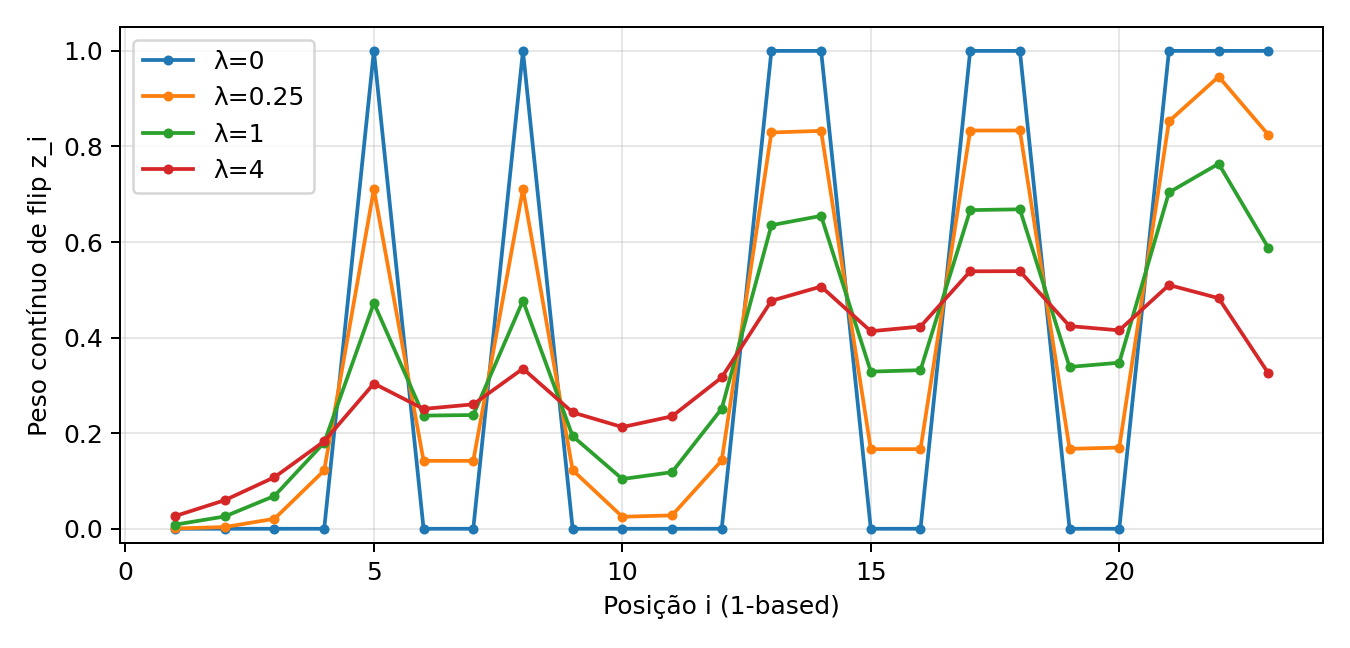
\includegraphics[width=\columnwidth]{resultados/grafico_pesos_flip.png}
\caption{Pesos contínuos de transformação. A penalização suaviza fronteiras e pode também alterar posições que não precisariam de flip.}
\end{figure}
\section{Análise complementar}
A diferença de escala na exploração dos grafos é visível na Figura~\ref{fig:exp}: a BFS visita muitas possibilidades de mesmo custo antes de chegar ao estado-alvo; a busca gulosa explícita prioriza as mais promissoras usando $h$. Em $L=16$, a BFS gerou, em média, $3.855.400,53$ sucessores (incluindo duplicatas), contra $544$ da Best-First. A versão otimizada evita inteiramente a materialização desses sucessores, mas não deve ter sua contagem lógica de etapas confundida com estados da árvore de busca.
\begin{figure}[h]
\centering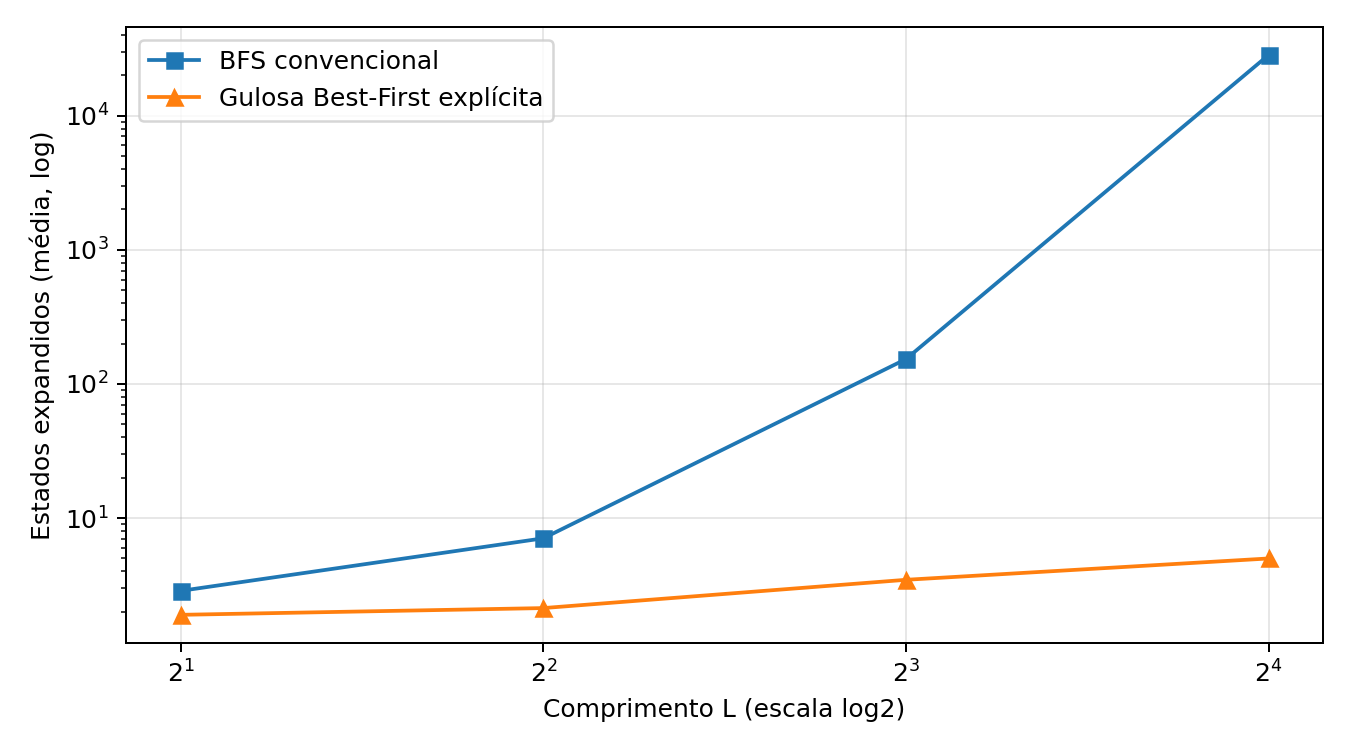
\includegraphics[width=\columnwidth]{resultados/grafico_expandidos.png}
\caption{Estados expandidos medidos apenas nos quatro menores comprimentos.}\label{fig:exp}
\end{figure}
A Figura~\ref{fig:gd} registra a queda de $J(x^{(k)})-J(x^{(\mathrm{final})})$ para todos os valores de $\lambda$, com passos adaptados à curvatura máxima da função quadrática. Todas as execuções partem de $J(x^{(0)})=9$, pois $z(x^{(0)})=0$; a Tabela~\ref{tab:gd} decompõe os resultados finais em fidelidade e regularização. A busca discreta ótima e a relaxação contínua respondem a perguntas diferentes: a primeira exige alcançar exatamente $t$ com custo inteiro mínimo, enquanto a segunda admite sacrificar fidelidade para obter um perfil de alterações espacialmente mais suave.
\begin{figure}[h]
\centering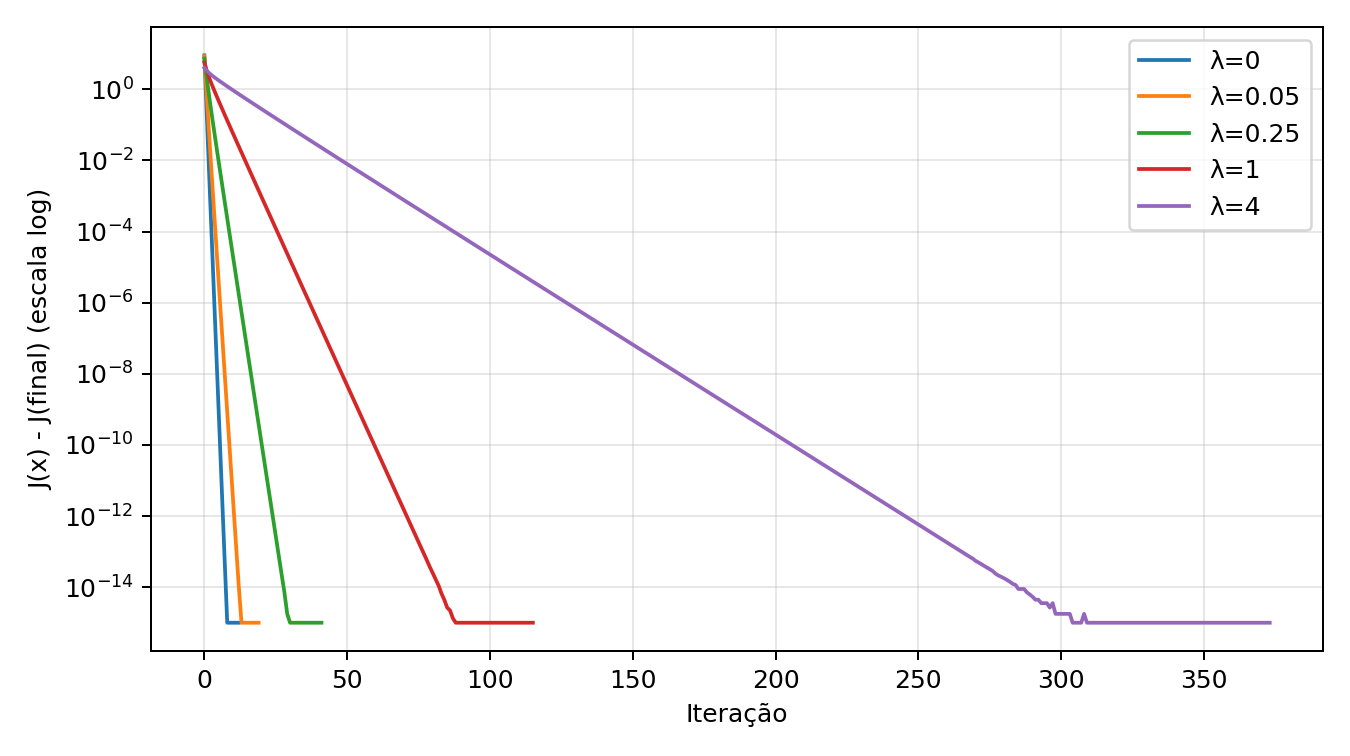
\includegraphics[width=\columnwidth]{resultados/grafico_gradiente.png}
\caption{Diferença entre o objetivo atual e o valor final numérico, com gradiente descendente projetado.}\label{fig:gd}
\end{figure}
\textbf{Verificação de implementação.} Além da comparação exaustiva entre as três buscas para os 256 pares possíveis de estados com quatro bits, derivadas analíticas de $J$ foram comparadas com diferenças finitas centrais, e foi verificado que a trajetória projetada permanece em $[0,1]^L$ e reduz o objetivo nos valores experimentados de $\lambda$.

\Needspace{9\baselineskip}
\section*{Reprodutibilidade}
Os arquivos \texttt{mini\_projeto.py}, \texttt{README.md}, CSVs, gráficos e \texttt{relatorio.tex} acompanham o material. Executar \texttt{python mini\_projeto.py --todos}. Há testes com os 256 pares possíveis de 4 bits e verificação do gradiente por diferenças finitas. \textbf{Repositório Git:} inserir URL real após publicar os arquivos (nenhum endereço externo foi presumido).
\end{document}
